% 2009 年福建卷理科第 18 题：赛道曲线 OSM 与折线 MNP。
% 来源 PDF：普通高考/2009/2009福建理.pdf，SHA-256 44d650687de50fff3efc1d37624b1272c9045e96d41491464f6713a708f202b9。
% 原页：第 2 页（A3 三栏）第 1 栏上部，书页码 516。
% 重绘依据：y=2√3 sin(πx/6)，x∈[0,4]；S(3,2√3)、M(4,3)、N(4+√3,0)、P(8,0)。
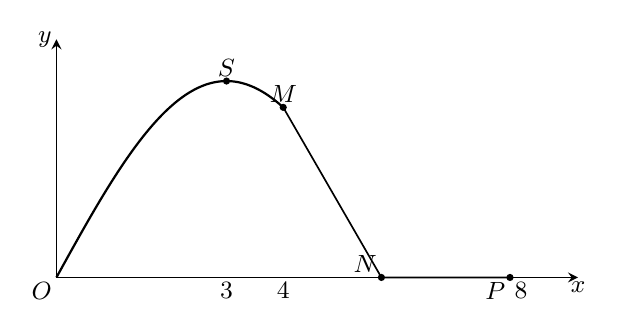
\begin{tikzpicture}[semithick, x=0.72cm, y=0.72cm, every node/.style={inner sep=1.4pt, font=\small}]
  \draw[-stealth] (0,0) -- (9.2,0) node[below] {$x$};
  \draw[-stealth] (0,0) -- (0,4.2) node[left] {$y$};
  \node[below left] at (0,0) {$O$};
  \draw[thick,domain=0:4,samples=100] plot (\x,{2*sqrt(3)*sin(30*\x)});
  \coordinate (S) at (3,3.464);
  \coordinate (M) at (4,3);
  \coordinate (N) at (5.732,0);
  \coordinate (P) at (8,0);
  \fill (S) circle (1.3pt);
  \fill (M) circle (1.3pt);
  \fill (N) circle (1.3pt);
  \fill (P) circle (1.3pt);
  \draw (M) -- (N) -- (P);
  \node[above] at (S) {$S$};
  \node[above] at (M) {$M$};
  \node[above left] at (N) {$N$};
  \node[below left] at (P) {$P$};
  \node[below] at (3,0) {$3$};
  \node[below] at (4,0) {$4$};
  \node[below right] at (8,0) {$8$};
\end{tikzpicture}
